\documentclass{article}
\usepackage[utf8]{inputenc}
\usepackage[english]{babel}
\usepackage{caption}
\usepackage[export]{adjustbox}
%\usepackage{comment}
\usepackage{hyperref}
\usepackage{graphicx}
% \usepackage{fancyhdr}
% \pagestyle{fancy}
% \fancyhf{}
% \fancyhead[R]{\thepage}
\usepackage{amsmath}
%\usepackage{authblk}
\graphicspath{{images/}}
\usepackage{geometry}
\usepackage[utf8]{inputenc}
\usepackage{array}
\usepackage{color,soul}
\pagenumbering{roman}
\usepackage{tabularx}
 \geometry{
 a4paper,
 total={170mm,257mm},
 left=15mm,
 top=10mm,
 bottom=2mm,
 }
\begin{document}
\setcounter{page}{8}

\begin{itemize}
\item \textbf{MIOU accuracy and Loss:}
The following are the graphs of MIOU accuracy and categorical cross entropy loss with respect to number of EPOCHS. The left half of the graph represents the result of training and the right half is for validation.

\begin{figure}[h]
    \centering
    \captionsetup{justification=centering}
    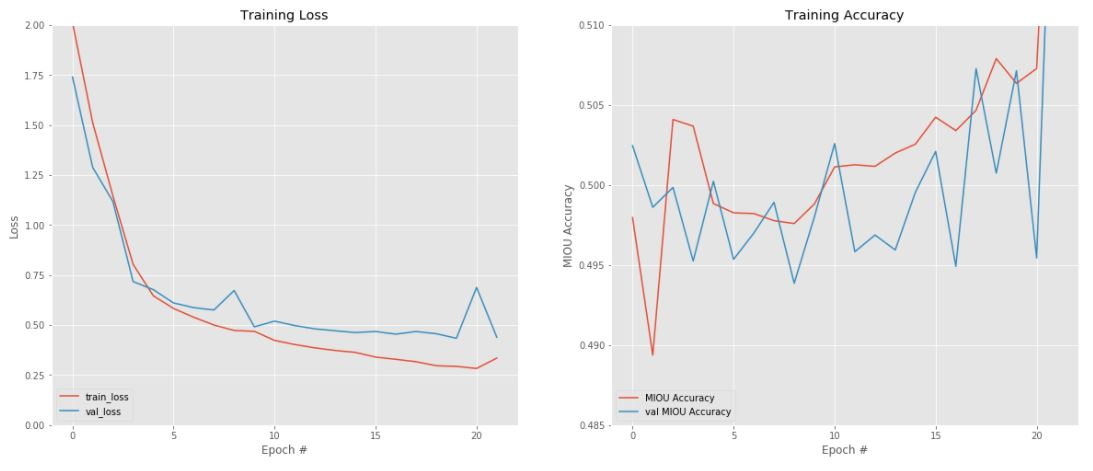
\includegraphics[width=14cm]{U-net-cityscrapes-B16-gr.JPG}
    \caption{U-net MIOU accuracy and Loss}
    \label{fig:Binary class segmented output}
\end{figure}

\begin{figure}[h]
    \centering
    \captionsetup{justification=centering}
    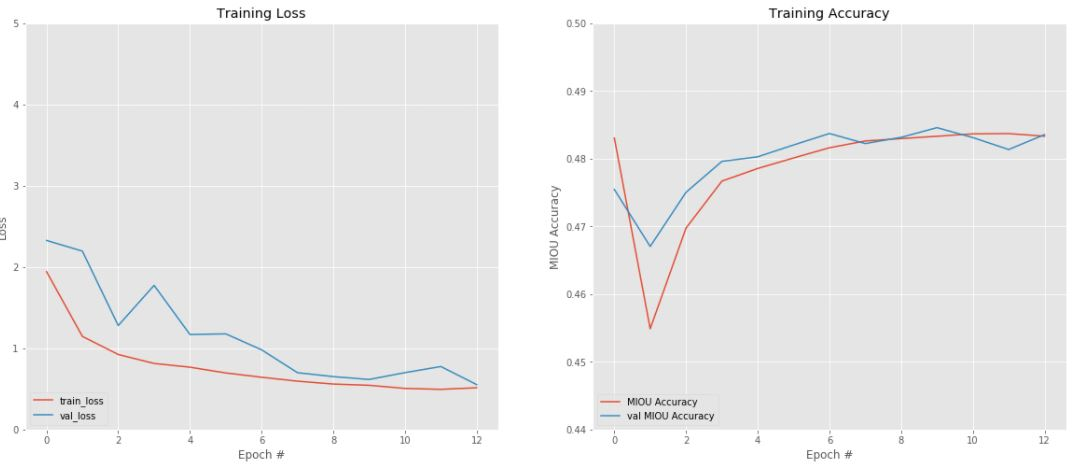
\includegraphics[width=14cm]{Segnet-cityscrapes-B16-gr.JPG}
    \caption{Segnet MIOU accuracy and Loss}
    \label{fig:Binary class segmented output}
\end{figure}

\begin{figure}[h]
    \centering
    \captionsetup{justification=centering}
    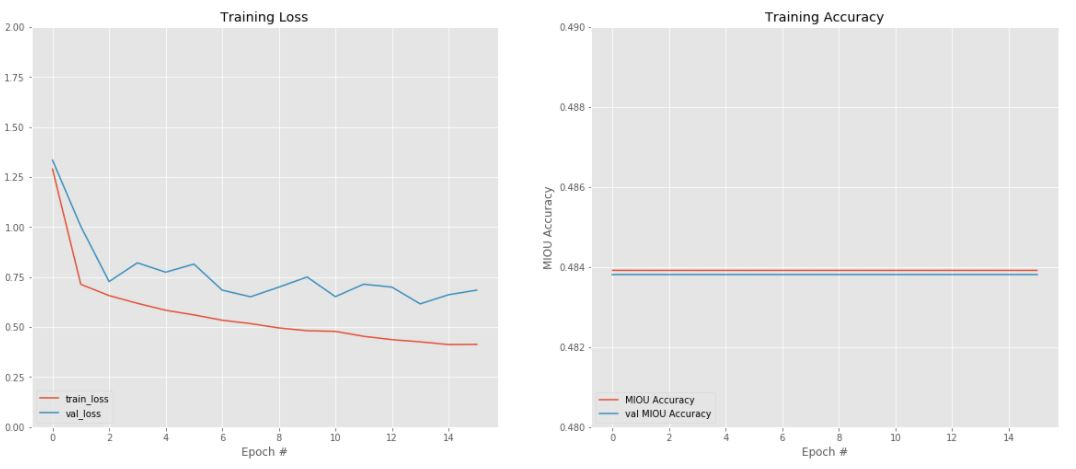
\includegraphics[width=14cm]{ICnet-cityscrapes-B16-gr.JPG}
    \caption{ICnet MIOU accuracy and Loss}
    \label{fig:Binary class segmented output}
\end{figure}

\begin{figure}[h]
    \centering
    \captionsetup{justification=centering}
    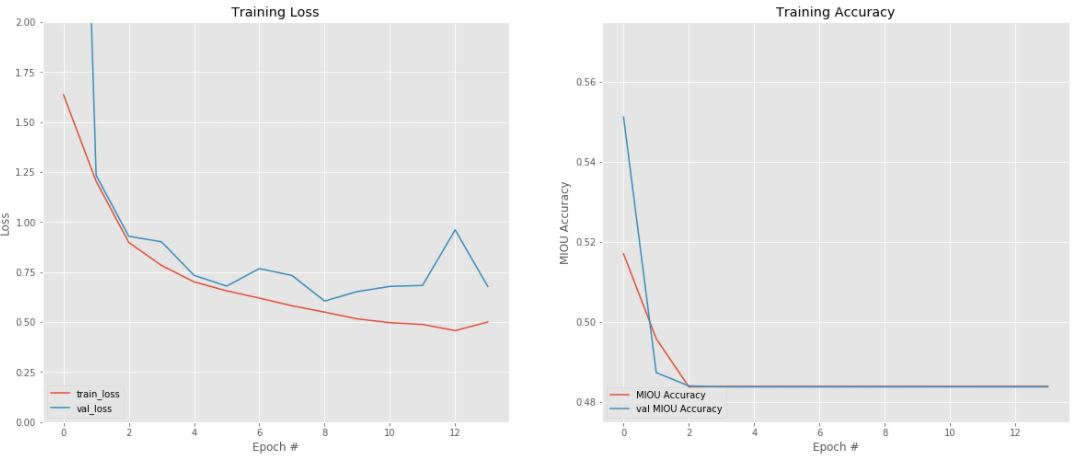
\includegraphics[width=14cm]{Resnet-cityscrapes-B16-gr.JPG}
    \caption{Resnet MIOU accuracy and Loss}
    \label{fig:Binary class segmented output}
\end{figure}
\newpage

\item \textbf{Precision vs Recall Graph:}
The following are the graphs of Precision vs Recall for 4 architectures. The left half of the graph represents the result of training and the right half is for validation.

\begin{figure}[h]
    \centering
    \captionsetup{justification=centering}
    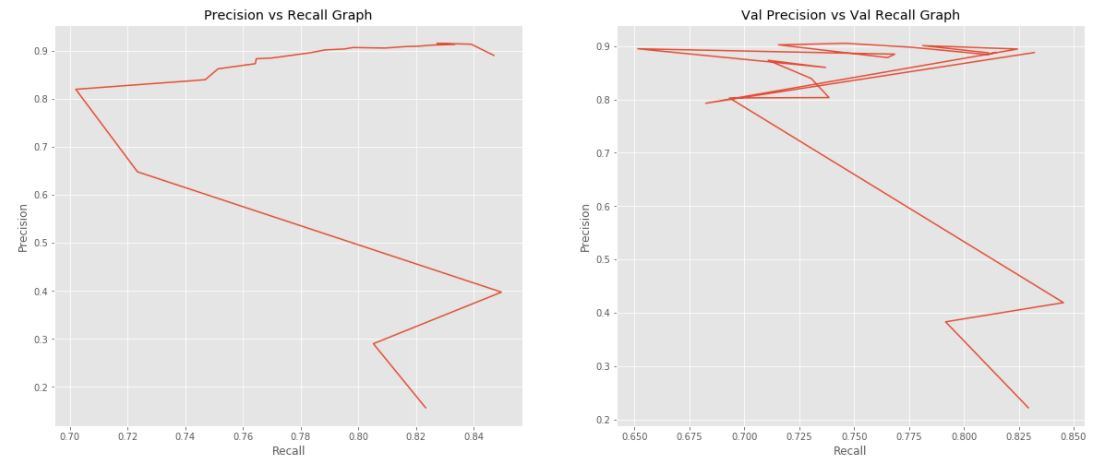
\includegraphics[width=14.5cm]{U-net-cityscrapes-B16-p-vs-re.JPG}
    \caption{U-net Precision vs Recall Graph}
    \label{fig:Binary class segmented output}
\end{figure}

\begin{figure}[h]
    \centering
    \captionsetup{justification=centering}
    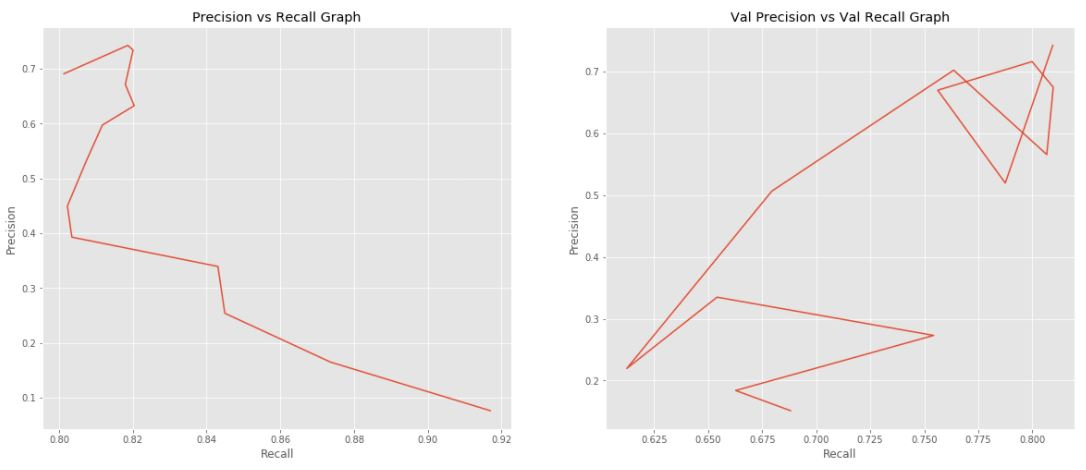
\includegraphics[width=14.5cm]{Segnet-cityscrapes-B16-p-vs-re.JPG}
    \caption{Segnet Precision vs Recall Graph}
    \label{fig:Binary class segmented output}
\end{figure}

\begin{figure}[h]
    \centering
    \captionsetup{justification=centering}
    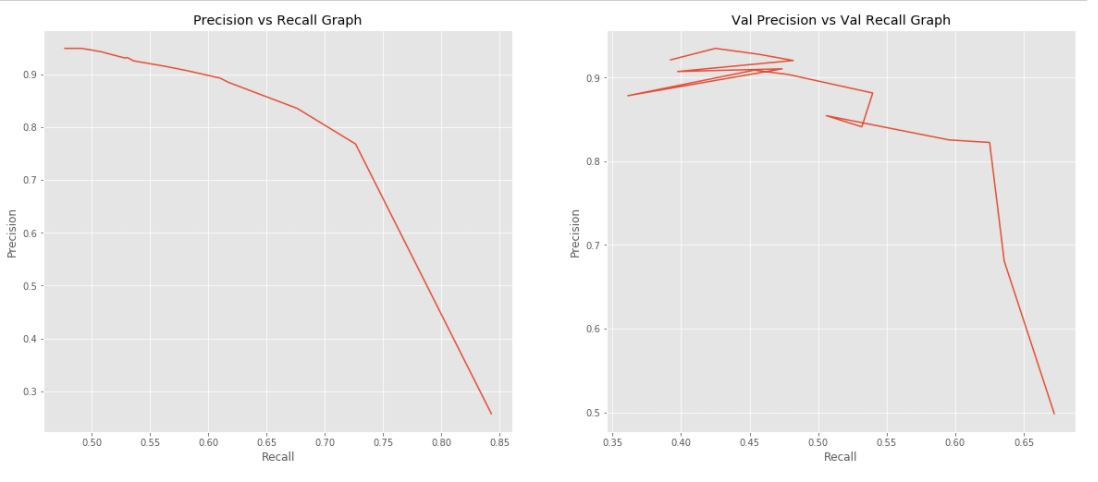
\includegraphics[width=15cm]{ICnet-cityscrapes-B16-p-vs-re.JPG}
    \caption{ICnet Precision vs Recall Graph}
    \label{fig:Binary class segmented output}
\end{figure}

\begin{figure}[h]
    \centering
    \captionsetup{justification=centering}
    \includegraphics[width=15cm]{Resnet-cityscrapes-B16-p-vs-re.JPG}
    \caption{Resnet Precision vs Recall Graph}
    \label{fig:Binary class segmented output}
\end{figure}
\end{itemize}
\newpage

\end{document}